We now turn our attention to in-context learning for more complex function classes, namely sparse linear functions, decision trees, and two-layer ReLU neural networks. Here, we are back in the setting where the distribution of prompts during inference is same as that during training (except the setting of neural networks where we evaluate on linear functions as well).
The overall methodology remains the same: we sample random functions from these families and train a Transformer from scratch to approximate these functions given in-context examples. (See Appendix~\ref{app:baselines} for more details and baselines.) 

\paragraph{Sparse linear functions.}
First, we consider functions of the form $f(x) = w^\top x$ where $w \in \mathbb{R}^d$ and has exactly $s$ non-zero coordinates.
To sample a prompt $P = (x_1, f(x_1), \ldots, x_k,f(x_k), x_\text{query})$, we draw prompt inputs $x_i$ and $x_\text{query}$, and a weight vector $w$ from $N(0, I_d)$, and then zero out all but $s$ coordinates of $w$ uniformly at random. 
We choose $d = 20$ and $s = 3$.
In this setting, the least squares estimator is no longer optimal---one can perform better by leveraging the weight vector sparsity. 
One estimator that leverages sparsity is Lasso~\citep{tibshirani1996regression}, which involves solving the least squares objective with an $\ell_1$-norm regularizer for the weight vector.
We plot the performance of our model in Figure \ref{fig:sparsity}, and observe that it is also able to leverage sparsity, nearly matching the performance of Lasso. Our model achieves errors $0.58$ and $0.09$ while Lasso achieves errors $0.62$ and $0.08$ for $k = 5$ and $10$ respectively. Note that, unlike least squares, Lasso does not have a closed form expression and involves iterative minimization of the regularized objective, yet the Transformer is able to achieve comparable performance in a single forward pass.
% 5, 10, 20
% Transformer [0.5765025615692139, 0.09006276726722717, 0.004361466504633427]
% Lasso [0.6237253348032633, 0.08302272856235504, 0.00023118976969271898]

\begin{figure}[ht]
    \phantom{}
    \hfill
    \begin{subfigure}[b]{0.4\textwidth}
        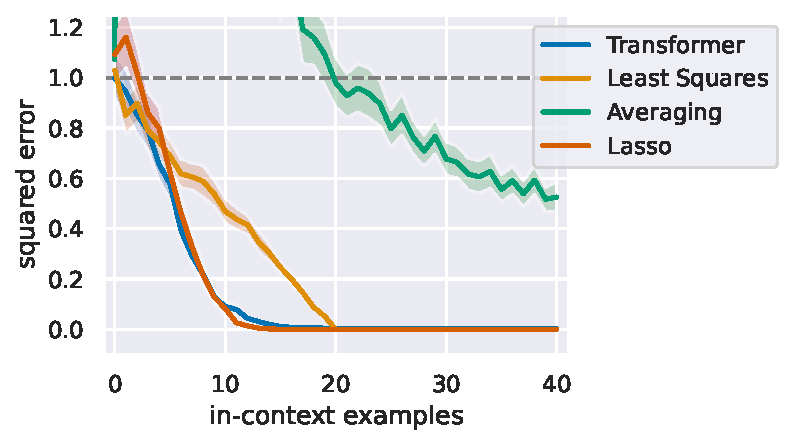
\includegraphics[height=.6\textwidth]{figures/sparsity.pdf}
        \caption{Sparse linear functions}
        \label{fig:sparsity}
    \end{subfigure}
    \hfill
    \begin{subfigure}[b]{0.4\textwidth}
        \centering
        %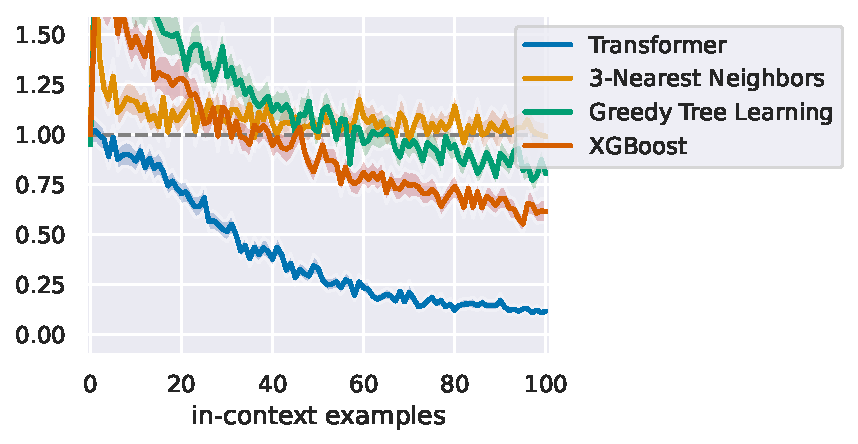
\includegraphics[height=.6\textwidth]{figures/tree.pdf}
        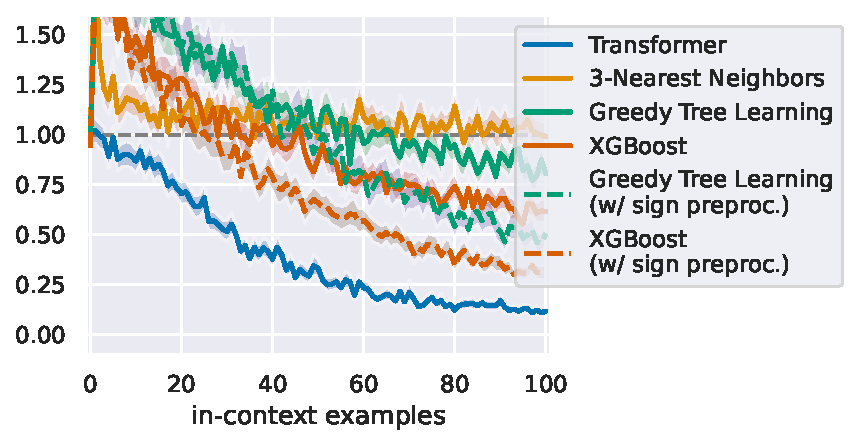
\includegraphics[height=.6\textwidth]{figures/tree_w_sign.pdf}
        \caption{Decision trees}
        \label{fig:decision_trees}
    \end{subfigure}
    \hfill
    \phantom{}
    \\
    \phantom{}
    \hfill
    \begin{subfigure}[b]{0.4\textwidth}
        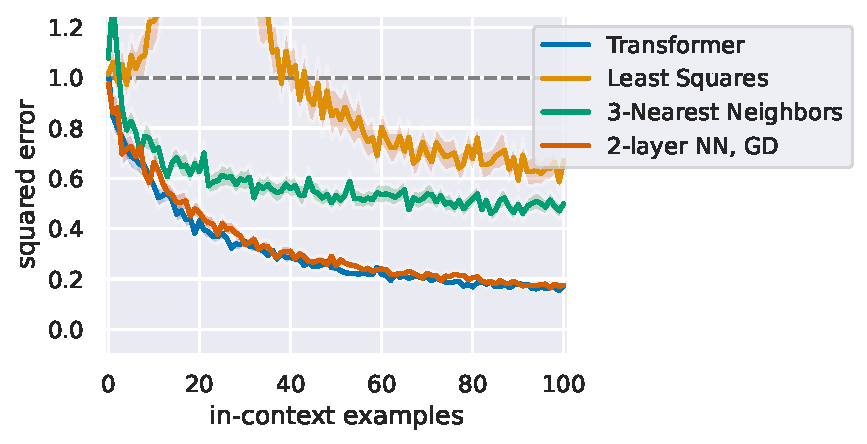
\includegraphics[height=.6\textwidth]{figures/relu.pdf}
        \caption{2-layer NN}
        \label{fig:relu}
    \end{subfigure}
    \hfill
    \begin{subfigure}[b]{0.4\textwidth}
        \centering
        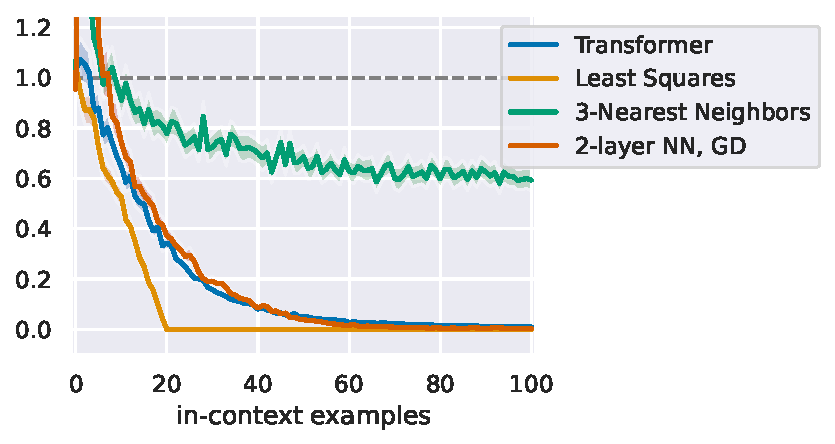
\includegraphics[height=.6\textwidth]{figures/relu_LR.pdf}
        \caption{2-layer NN, eval on linear functions}
        \label{fig:relu_lr}
    \end{subfigure}
    \hfill
    \phantom{}
    \caption{\emph{Training a Transformer  to in-context learn more complex function classes. } 
    (a) A Transformer trained on prompts generated using sparse linear functions can in-context learn this class, with error decreasing at a rate similar to Lasso, and significantly better than minimum norm least squares.
    (b) A Transformer trained on prompts generated using random decision trees can in-context learn this class, 
    with much better performance  than greedy tree learning or tree boosting.
    (c) A Transformer trained on prompts generated using random 2-layer ReLU neural networks can in-context learn this class. The error decreases at a rate similar to the baseline which involves training a neural network using a variant of gradient descent with in-context examples as the training data. (d) The same model (from (c)) can in-context learn the class of linear functions. The error decreases at a rate slower than least squares, but comparable to a neural network trained using a variant of gradient descent. In all cases, the errors are normalized so that the trivial zero estimator achieves an error of $1$ (dashed line).
    % \pl{(d) linear functions caption is confusing;
    % should say 2-layer NN (eval on linear) or something
    % }
    }
\end{figure}

\paragraph{Decision trees.} 
Next, we consider the class of depth 4 decision trees with 20 dimensional inputs. A function $f$ in this class is represented by a full binary tree (with 16 leaf nodes) where each non-leaf node is associated with a coordinate, and each leaf node is associated with a target value. To evaluate $f$ on an input $x$, we traverse the tree starting from the root node, and go to the right child if the coordinate associated with the current node is positive and go to the left child otherwise (that is, the threshold at each node is $0$). $f(x)$ is given by the value associated with the leaf node reached at the end. To sample a  random prompt $P = (x_1, f(x_1), \ldots, x_k, f(x_k), x_\text{query})$, we draw prompt inputs $x_i$s and $x_\text{query}$ from $N(0, I_d)$, and $f$ corresponds to a tree where the coordinates associated with the non-leaf nodes are drawn uniformly at random from $\{1, 2,  \ldots, d\}$ and the values associated with the leaf nodes are drawn from $N(0, 1)$. 
In Figure \ref{fig:decision_trees}, we show that Transformers can be trained to in-context learn this class, with performance much better than  greedy tree learning and boosting (via XGBoost~\citep{chen2016xgboost}).
With $k=100$ in-context examples, the Transformer achieves an error of $0.12$ whereas greedy learning achieves an error of $0.80$ and XGBoost achieves an error of $0.62$.
%Transformer [0.11640552431344986]
%Greedy Tree Learning [0.8047670125961304]
%Greedy (w/ sign) [0.5035423040390015]
%XGBoost [0.6160200238227844]
%XGBoost (w/ sign) [0.30775895714759827]

Since the decision trees in our function class predict solely based on the sign of each coordinate of $x_i$, we also consider a baseline where we provide the greedy learning and XGBoost algorithms with the signs of each $x_i$ instead. %SIGN
This significantly improves their performance---at 100 in-context examples, greedy achieves an error of 0.50 and XGBoost an error if 0.31---but they still perform much worse than the trained Transformer.

Note that, in general, we do not have a good understanding of the space of efficient algorithms for learning decision trees, and the conditions under which known heuristics work \citep{blanc2021decision, brutzkus2020id3}.
At the same time, we found that Transformers can be trained to directly discover such an algorithm for the prompt distribution we considered. This suggests an intriguing possibility where we might be able to reverse engineer the algorithm encoded by a Transformer to obtain new sample efficient algorithms for existing learning problems. 

\paragraph{Two-layer ReLU neural networks.}
Finally, we consider the class of two layer ReLU neural 
networks containing functions of the form $f(x) = \sum_{i=1}^r \alpha_i \ \sigma(w_i^\top x)$, where $\alpha_i \in \mathbb{R}$, $w_i \in \mathbb{R}^d$ and $\sigma(\cdot) = \max(0, \cdot)$ is the ReLU activation function.
To draw a random prompt $P = (x_1, f(x_1), \ldots, x_k, f(x_k), x_\text{query})$, we sample prompt inputs $x_i$s and $x_\text{query}$ from $N(0, I_d)$, along with network parameters $a_i$s and $w_i$s from $N(0, {2/r})$ and $N(0, I_d)$ respectively. We set the input dimension $d$ to $20$ and the number of the hidden nodes $r$ to $100$. 
In Figure~\ref{fig:relu}, we show that Transformers can be trained to in-context learn this class of functions.
In fact, the Transformer performs comparably to the baseline 
 which involves training a two-layer neural network of the same architecture on in-context examples using Adam \citep{kingma2014adam}, a variant of gradient descent
(see Appendix \ref{app:baselines} for details). Specifically, for $k=100$ in-context examples, both the Transformer and the neural network trained on in-context examples achieve an error of $0.17$.
%Transformer [0.4317147731781006, 0.24363529682159424, 0.17297804355621338]
%Least Squares [164167.35, 0.8709582328796387, 0.6713057041168213]
%3-Nearest Neighbors [0.6261932849884033, 0.5321125030517578, 0.49874200820922854]
%Averaging [1.6577213287353516, 1.0084754943847656, 0.7262303352355957]
%2-layer NN, GD, lr=0.005 [0.46292924880981445, 0.25183374881744386, 0.17450664043426514]



Moreover, the model trained to in-context learn two-layer neural networks is also able to in-context learn linear functions (for which it is not explicitly trained), albeit with a rate slower than least squares, but comparable to a neural network trained on in-context examples generated using a linear function (Figure \ref{fig:relu_lr}). For $k=20$, $50$, and $100$ in-context examples respectively, the Transformer achieves error $0.34$, $0.05$, and $0.01$, and the two-layer network achieves error $0.37$, $0.04$, and $0.003$ (the least squares estimator achieves error $0$ for $k\geq 20$).
%Transformer [0.34319705963134767, 0.05081412196159363, 0.009670931845903397]
%Least Squares [7.934294998790392e-10, 7.940695627081662e-14, 6.064989547908962e-14]
%3-Nearest Neighbors [0.7789178371429444, 0.686550521850586, 0.5931134223937988]
%Averaging [1.0506414413452148, 0.43355441093444824, 0.21713628768920898]
%2-layer NN, GD, lr=0.005 [0.38516089916229246, 0.0691907286643982, 0.012784336507320405]
%2-layer NN, GD, lr=0.05 [0.37147202491760256, 0.03918924033641815, 0.0029806846752762793]



